% move all configuration stuff into includes file so we can focus on the content
\documentclass[aspectratio=169,hyperref={pdfpagelabels=false,colorlinks=true,linkcolor=white,urlcolor=lightblue},xcolor={table},t]{beamer}

%%%%%%%%%%%%%%%%%%%%%%%%%%%%%%%%%%%%%%%%%%%%%%%%%%%%%%%%%%%%%%%%%%%%%%%%%%%%%%%%%%
%%%%%%%%%%%%%%%%%%%%%%%%%%%%%%%%%%%%%%%%%%%%%%%%%%%%%%%%%%%%%%%%%%%%%%%%%%%%%%%%%%
% packages
\usepackage{pict2e}
\usepackage{epic}
\usepackage{amsmath,amsfonts,amssymb}
\usepackage{units}
\usepackage{fancybox}
\usepackage[absolute,overlay]{textpos} 
%\usepackage[table]{xcolor}
\usepackage{animate}
\usepackage{gensymb}
%\usepackage{graphicx}
%\usepackage{longtable}
\usepackage{multirow}
\usepackage{silence}
\usepackage{tikz}
\usepackage[backend=bibtex,style=ieee]{biblatex}
\AtEveryCitekey{\iffootnote{\tiny}{}}
\addbibresource{include/references}



% fontsize
\let\Tiny=\tiny

%%%%%%%%%%%%%%%%%%%%%%%%%%%%%%%%%%%%%%%%%%%%%%%%%%%%%%%%%%%%%%%%%%%%%%%%%%%%%%%%%%
%%%%%%%%%%%%%%%%%%%%%%%%%%%%%%%%%%%%%%%%%%%%%%%%%%%%%%%%%%%%%%%%%%%%%%%%%%%%%%%%%%
% warnings
\pdfsuppresswarningpagegroup=1
\WarningFilter{biblatex}{Patching footnotes failed}
\WarningFilter{latexfont}{Font shape}
\WarningFilter{latexfont}{Some font shapes}
\WarningFilter{gensymb}{Not defining}


%%%%%%%%%%%%%%%%%%%%%%%%%%%%%%%%%%%%%%%%%%%%%%%%%%%%%%%%%%%%%%%%%%%%%%%%%%%%%%%%%%
%%%%%%%%%%%%%%%%%%%%%%%%%%%%%%%%%%%%%%%%%%%%%%%%%%%%%%%%%%%%%%%%%%%%%%%%%%%%%%%%%%
% theme & layout
\usetheme{Frankfurt}
\useinnertheme{rectangles}


%%%%%%%%%%%%%%%%%%%%%%%%%%%%%%%%%%%%%%%%%%%%%%%%%%%%%%%%%%%%%%%%%%%%%%%%%%%%%%%%%%
\setbeamertemplate{frametitle}[default][colsep=-4bp,rounded=false,shadow=false]
\setbeamertemplate{frametitle}
{%
    \nointerlineskip%
    %\vskip-0.5ex
    \begin{beamercolorbox}[wd=\paperwidth,ht=3.5ex,dp=0.6ex]{frametitle}
        \hspace*{1.3ex}\insertframetitle%
        
        \hspace*{1.3ex}\small\insertframesubtitle%
    \end{beamercolorbox}%
    \begin{textblock*}{100mm}(13.75cm,1cm)
        
\includegraphics[height=.4cm,keepaspectratio]{graph/Logo_GTCMT_white}
    \end{textblock*}
}


%%%%%%%%%%%%%%%%%%%%%%%%%%%%%%%%%%%%%%%%%%%%%%%%%%%%%%%%%%%%%%%%%%%%%%%%%%%%%%%%%%
\setbeamertemplate{title page}[default][colsep=-4bp,rounded=false,shadow=false]
\setbeamertemplate{title page}
{
    \begin{textblock*}{100mm}(15cm,.51cm)
            \href{https://github.com/alexanderlerch/ACA-Slides/blob/2nd_edition/\jobname.pdf}{\includegraphics[height=.5cm,keepaspectratio]{graph/Logo_github}}\hspace*{2ex}
    \end{textblock*}
    \begin{textblock*}{100mm}(15cm,1.3cm)
            \href{\IEEELink}{
\includegraphics[height=.5cm,keepaspectratio]{graph/icon/book}}\hspace*{2ex}
    \end{textblock*}
    \vskip-10ex
    \begin{beamercolorbox}[wd=\paperwidth,ht=.7\paperheight,dp=0.6ex]{frametitle} %35ex
        %\begin{flushright}
            %\href{http://www.gtcmt.gatech.edu}{
\includegraphics[height=.8cm,keepaspectratio]{graph/Logo_GTCMT_black}}\hspace*{2ex}
        %\end{flushright}
        
        \hspace*{1.8ex}\LARGE\inserttitle%
        
        \vspace*{.5ex}
        
        \hspace*{1.3ex}\small\insertsubtitle%
        
        \vspace*{.5ex}
    \end{beamercolorbox}%
    \nointerlineskip%
    \begin{beamercolorbox}[wd=\paperwidth,ht=.4\paperheight,dp=0.6ex]{page number in head/foot}
        %\vspace*{-.5ex}
        \hspace*{1.7ex}\small\insertauthor%
        
        %\hspace*{1.7ex}\small }%
        
        \vspace*{12ex}
        \vfill
        \begin{flushright}
            \href{http://www.gtcmt.gatech.edu}{
\includegraphics[height=.5cm,keepaspectratio]{graph/Logo_GTCMT_black}}\hspace*{2ex}
        \end{flushright}
    \end{beamercolorbox}%
}


%%%%%%%%%%%%%%%%%%%%%%%%%%%%%%%%%%%%%%%%%%%%%%%%%%%%%%%%%%%%%%%%%%%%%%%%%%%%%%%%%%
%\makeatother
\setbeamertemplate{footline}
{
  \leavevmode%
  \hbox{%
  \begin{beamercolorbox}[wd=.5\paperwidth,ht=2.25ex,dp=1ex,left,leftskip=1ex]{page number in head/foot}%
    \insertsubtitle
  \end{beamercolorbox}%
  \begin{beamercolorbox}[wd=.5\paperwidth,ht=2.25ex,dp=1ex,right,rightskip=1ex]{page number in head/foot}%
    \hfill
    \insertframenumber{} / \inserttotalframenumber
  \end{beamercolorbox}}%
  \vskip0pt%
}
%\makeatletter


%%%%%%%%%%%%%%%%%%%%%%%%%%%%%%%%%%%%%%%%%%%%%%%%%%%%%%%%%%%%%%%%%%%%%%%%%%%%%%%%%%
\beamertemplatenavigationsymbolsempty
\setbeamertemplate{navigation symbols}{}
\setbeamertemplate{blocks}[default]%[rounded=false,shadow=false]
\setbeamertemplate{itemize item}[square]
\setbeamertemplate{itemize subitem}[circle]
\setbeamertemplate{itemize subsubitem}[triangle]
\setbeamertemplate{enumerate item}[square]
\setbeamertemplate{enumerate subitem}[circle]
\setbeamertemplate{enumerate subsubitem}[circle]


%%%%%%%%%%%%%%%%%%%%%%%%%%%%%%%%%%%%%%%%%%%%%%%%%%%%%%%%%%%%%%%%%%%%%%%%%%%%%%%%%%
% colors
\setbeamercolor{structure}{fg=darkgray}
\setbeamercovered{transparent} %invisible
\setbeamercolor{bibliography entry author}{fg=black}
\setbeamercolor*{bibliography entry title}{fg=black}
\setbeamercolor*{bibliography entry note}{fg=black}
\setbeamercolor{frametitle}{fg=black}
\setbeamercolor{title}{fg=white}
\setbeamercolor{subtitle}{fg=white}
\setbeamercolor{frametitle}{fg=white}
\setbeamercolor{framesubtitle}{fg=white}
\setbeamercolor{mini frame}{fg=white, bg=black}
\setbeamercolor{section in head/foot}{fg=white, bg=darkgray}
\setbeamercolor{page number in head/foot}{fg=black, bg=lightblue}
\setbeamercolor{item projected}{fg=white, bg=black}

%---------------------------------------------------------------------------------
%%%%%%%%%%%%%%%%%%%%%%%%%%%%%%%%%%%%%%%%%%%%%%%%%%%%%%%%%%%%%%%%%%%%%%%%%%%%%%%%%%
%%%%%%%%%%%%%%%%%%%%%%%%%%%%%%%%%%%%%%%%%%%%%%%%%%%%%%%%%%%%%%%%%%%%%%%%%%%%%%%%%%
% title information
\title[]{Introduction to \textbf{Audio Content Analysis}}   
\author[alexander lerch]{alexander lerch} 
%\institute{~}
%\date[Alexander Lerch]{}
%\titlegraphic{\vspace{-16mm}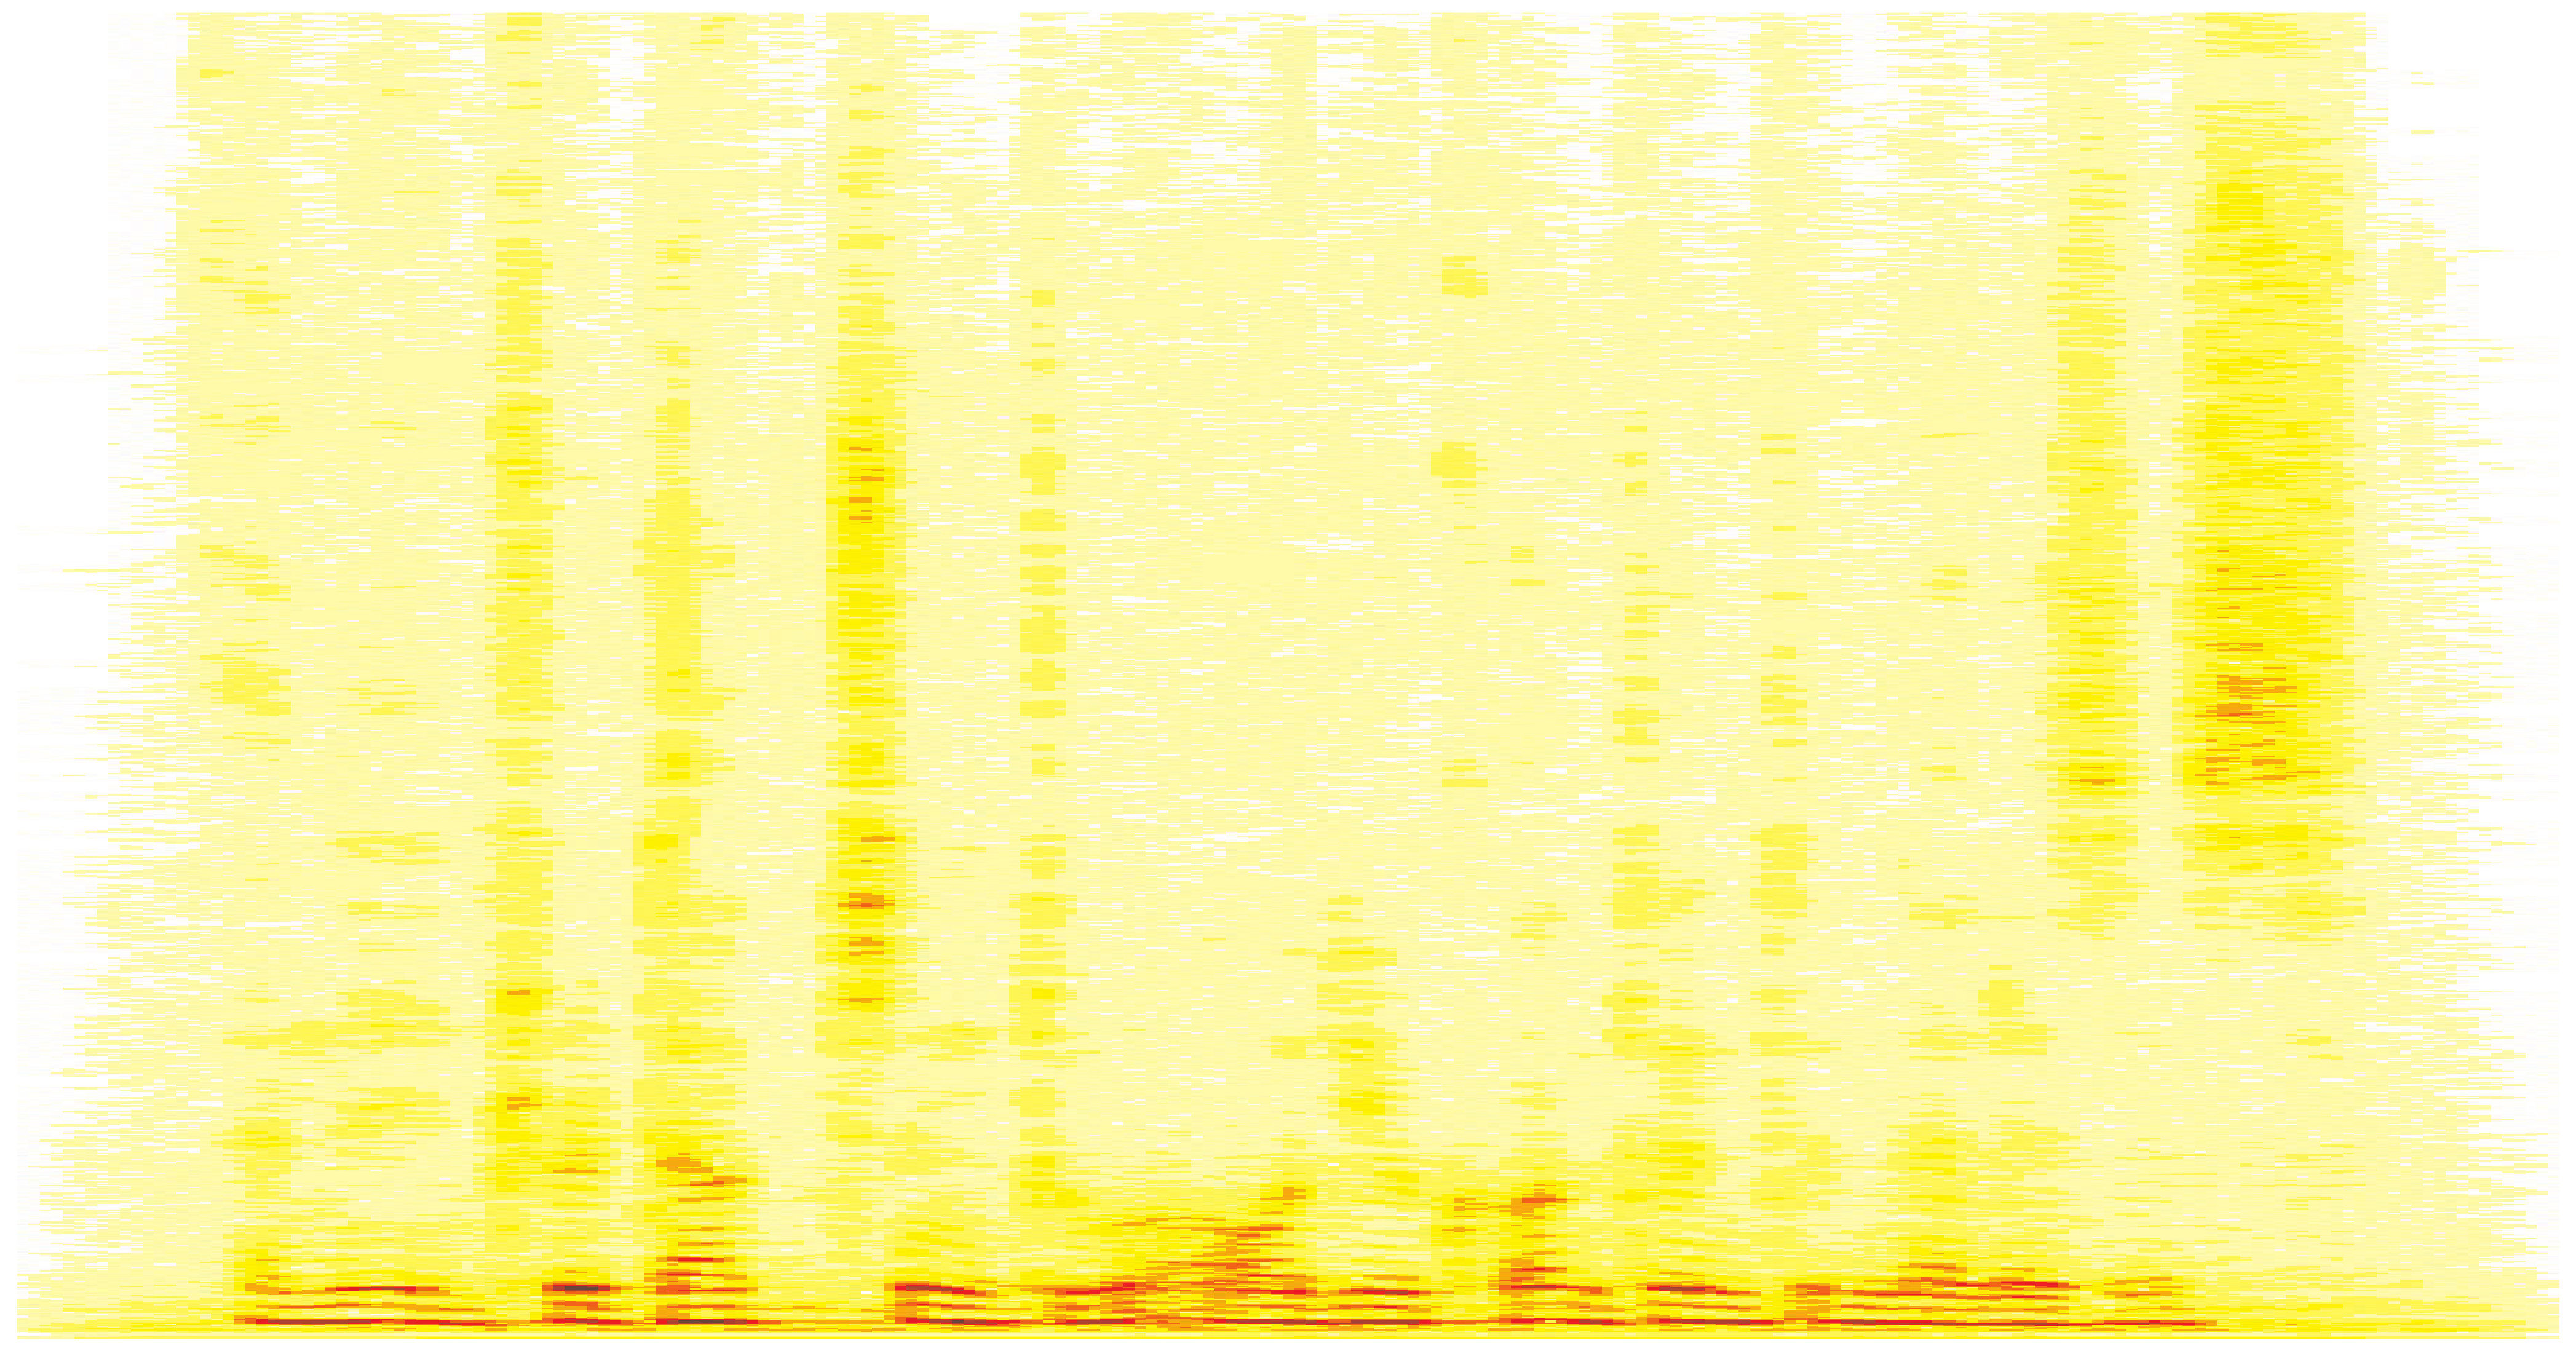
\includegraphics[width=\textwidth,height=3cm]{title}}

%%%%%%%%%%%%%%%%%%%%%%%%%%%%%%%%%%%%%%%%%%%%%%%%%%%%%%%%%%%%%%%%%%%%%%%%%%%%%%%%%%
%%%%%%%%%%%%%%%%%%%%%%%%%%%%%%%%%%%%%%%%%%%%%%%%%%%%%%%%%%%%%%%%%%%%%%%%%%%%%%%%%%
% colors
\definecolor{gtgold}{HTML}{96caff} %0e7eed {rgb}{0.88,0.66,1,0.06} [234, 170, 0]/256
\definecolor{darkgray}{rgb}{.1, .1, .25}
\definecolor{lightblue}{HTML}{0e7eed}
\definecolor{highlight}{rgb}{0, 0, 1} %_less!40

%%%%%%%%%%%%%%%%%%%%%%%%%%%%%%%%%%%%%%%%%%%%%%%%%%%%%%%%%%%%%%%%%%%%%%%%%%%%%%%%%%
%%%%%%%%%%%%%%%%%%%%%%%%%%%%%%%%%%%%%%%%%%%%%%%%%%%%%%%%%%%%%%%%%%%%%%%%%%%%%%%%%%
% relative paths
\graphicspath{{../ACA-Plots/graph/}}


%%%%%%%%%%%%%%%%%%%%%%%%%%%%%%%%%%%%%%%%%%%%%%%%%%%%%%%%%%%%%%%%%%%%%%%%%%%%%%%%%%
%%%%%%%%%%%%%%%%%%%%%%%%%%%%%%%%%%%%%%%%%%%%%%%%%%%%%%%%%%%%%%%%%%%%%%%%%%%%%%%%%%
% units
\setlength{\unitlength}{1mm}

%%%%%%%%%%%%%%%%%%%%%%%%%%%%%%%%%%%%%%%%%%%%%%%%%%%%%%%%%%%%%%%%%%%%%%%%%%%%%%%%%%
%%%%%%%%%%%%%%%%%%%%%%%%%%%%%%%%%%%%%%%%%%%%%%%%%%%%%%%%%%%%%%%%%%%%%%%%%%%%%%%%%%
% math
\DeclareMathOperator*{\argmax}{argmax}
\DeclareMathOperator*{\argmin}{argmin}
\DeclareMathOperator*{\atan}{atan}
\DeclareMathOperator*{\arcsinh}{arcsinh}
\DeclareMathOperator*{\sign}{sign}
\DeclareMathOperator*{\tcdf}{tcdf}
\DeclareMathOperator*{\si}{sinc}
\DeclareMathOperator*{\princarg}{princarg}
\DeclareMathOperator*{\arccosh}{arccosh}
\DeclareMathOperator*{\hwr}{HWR}
\DeclareMathOperator*{\flip}{flip}
\DeclareMathOperator*{\sinc}{sinc}
\DeclareMathOperator*{\floor}{floor}
\newcommand{\e}{{e}}
\newcommand{\jom}{\mathrm{j}\omega}
\newcommand{\jOm}{\mathrm{j}\Omega}
\newcommand   {\mat}[1]    		{\boldsymbol{\uppercase{#1}}}		%bold
\renewcommand {\vec}[1]    		{\boldsymbol{\lowercase{#1}}}		%bold

%%%%%%%%%%%%%%%%%%%%%%%%%%%%%%%%%%%%%%%%%%%%%%%%%%%%%%%%%%%%%%%%%%%%%%%%%%%%%%%%%%
%%%%%%%%%%%%%%%%%%%%%%%%%%%%%%%%%%%%%%%%%%%%%%%%%%%%%%%%%%%%%%%%%%%%%%%%%%%%%%%%%%
% media9
\newcommand{\includeaudio}[1]{
\href{run:audio/#1.mp3}{
\includegraphics[width=5mm, height=5mm]{graph/SpeakerIcon}}}

\newcommand{\includeanimation}[4]{{\begin{center}
                        \animategraphics[autoplay,loop,scale=.7]{#4}{animation/#1-}{#2}{#3}        
                        \end{center}
                        \addreference{matlab source: \href{https://github.com/alexanderlerch/ACA-Plots/blob/master/matlab/animate#1.m}{matlab/animate#1.m}}}
                        \inserticon{video}}
                        
%%%%%%%%%%%%%%%%%%%%%%%%%%%%%%%%%%%%%%%%%%%%%%%%%%%%%%%%%%%%%%%%%%%%%%%%%%%%%%%%%%
%%%%%%%%%%%%%%%%%%%%%%%%%%%%%%%%%%%%%%%%%%%%%%%%%%%%%%%%%%%%%%%%%%%%%%%%%%%%%%%%%%
% other commands
\newcommand{\question}[1]{%\vspace{-4mm}
                          \setbeamercovered{invisible}
                          \begin{columns}[T]
                            \column{.9\textwidth}
                                \textbf{#1}
                            \column{.1\textwidth}
                                \vspace{-8mm}
                                \begin{flushright}
                                     
\includegraphics[width=.9\columnwidth]{graph/question_mark}
                                \end{flushright}
                                \vspace{6mm}
                          \end{columns}\pause\vspace{-12mm}}

\newcommand{\toremember}[1]{
                        \inserticon{lightbulb}
                        }

\newcommand{\matlabexercise}[1]{%\vspace{-4mm}
                          \setbeamercovered{invisible}
                          \begin{columns}[T]
                            \column{.8\textwidth}
                                \textbf{matlab exercise}: #1
                            \column{.2\textwidth}
                                \begin{flushright}
                                     
\includegraphics[scale=.5]{graph/logo_matlab}
                                \end{flushright}
                                %\vspace{6mm}
                          \end{columns}}

\newcommand{\addreference}[1]{  
                  
                    \begin{textblock*}{\baselineskip }(.98\paperwidth,.5\textheight) %(1.15\textwidth,.4\textheight)
                         \begin{minipage}[b][.5\paperheight][b]{1cm}%
                            \vfill%
                             \rotatebox{90}{\tiny {#1}}
                        \end{minipage}
                   \end{textblock*}
                    }
                    
\newcommand{\figwithmatlab}[1]{
                    \begin{figure}
                        \centering
                        \includegraphics[scale=.7]{#1}
                        %\label{fig:#1}
                    \end{figure}
                    
                    \addreference{matlab source: \href{https://github.com/alexanderlerch/ACA-Plots/blob/main/matlab/plot#1.m}{plot#1.m}}}
\newcommand{\figwithref}[2]{
                    \begin{figure}
                        \centering
                        \includegraphics[scale=.7]{#1}
                        \label{fig:#1}
                    \end{figure}
                    
                    \addreference{#2}}  
                                    
\newcommand{\inserticon}[1]{
                    \begin{textblock*}{100mm}(14.5cm,7.5cm)
                        \includegraphics[height=.8cm,keepaspectratio]{graph/#1}
                    \end{textblock*}}            

%%%%%%%%%%%%%%%%%%%%%%%%%%%%%%%%%%%%%%%%%%%%%%%%%%%%%%%%%%%%%%%%%%%%%%%%%%%%%%%%%%
%%%%%%%%%%%%%%%%%%%%%%%%%%%%%%%%%%%%%%%%%%%%%%%%%%%%%%%%%%%%%%%%%%%%%%%%%%%%%%%%%%
% counters
\newcounter{i}
\newcounter{j}
\newcounter{iXOffset}
\newcounter{iYOffset}
\newcounter{iXBlockSize}
\newcounter{iYBlockSize}
\newcounter{iYBlockSizeDiv2}
\newcounter{iXBlockSizeDiv2}
\newcounter{iDistance}

\newcommand{\IEEELink}{https://ieeexplore.ieee.org/servlet/opac?bknumber=9965970}




\subtitle{module 7.5: musical key recognition}

%%%%%%%%%%%%%%%%%%%%%%%%%%%%%%%%%%%%%%%%%%%%%%%%%%%%%%%%%%%%%%%%%%%%%%%%%%%%
\begin{document}
    % generate title page
	{
\setbeamertemplate{headline}{} 
\setbeamertemplate{footline}{} 
\begin{frame}
    \titlepage
    %\vspace{-5mm}
\end{frame}
}
\addtocounter{framenumber}{-1}


    \section[overview]{lecture overview}
        \begin{frame}{introduction}{overview}
            \begin{block}{corresponding textbook section}
                    %\href{http://ieeexplore.ieee.org/xpl/articleDetails.jsp?arnumber=6331122}{Chapter 5~---~Tonal Analysis}: pp.~88--94\\
                    %\href{http://ieeexplore.ieee.org/xpl/articleDetails.jsp?arnumber=6331122}{Chapter 5~---~Tonal Analysis}: pp.~116--125
                    section~7.5
            \end{block}

            \begin{itemize}
                \item   \textbf{lecture content}
                    \begin{itemize}
                        \item   definition of musical key
                        \item   pitch chroma feature
                        \item   standard approach for key recognition
                    \end{itemize}
                \bigskip
                \item<2->   \textbf{learning objectives}
                    \begin{itemize}
                        \item   explain the defining properties of a musical key
                        \item   implement a simple pitch chroma feature extractor
                        \item   describe and  discuss a simple automatic key recognition system
                    \end{itemize}
            \end{itemize}
            \inserticon{directions}
        \end{frame}

    \section{key}
        \begin{frame}{key}{tonic \& mode}
            \begin{columns}
            \column{0.38\linewidth}
            \begin{itemize}
                \item	\textbf{tonic}: first scale degree
                        \begin{itemize}
                            \item	most ``important'' pitch class
                        \end{itemize}
                
                \item	\textbf{mode}: set of diatonic pitch relationships
                        \begin{itemize}
                            \item	Major: 2, 2, 1, 2, 2, 2, 1
                            \item	Minor: 2, 1, 2, 2, 1, 2, 2
                        \end{itemize}
            \end{itemize}
            \column{0.5\linewidth}
                \vspace{-10mm}
                \begin{figure}[t]
                    \centering
                    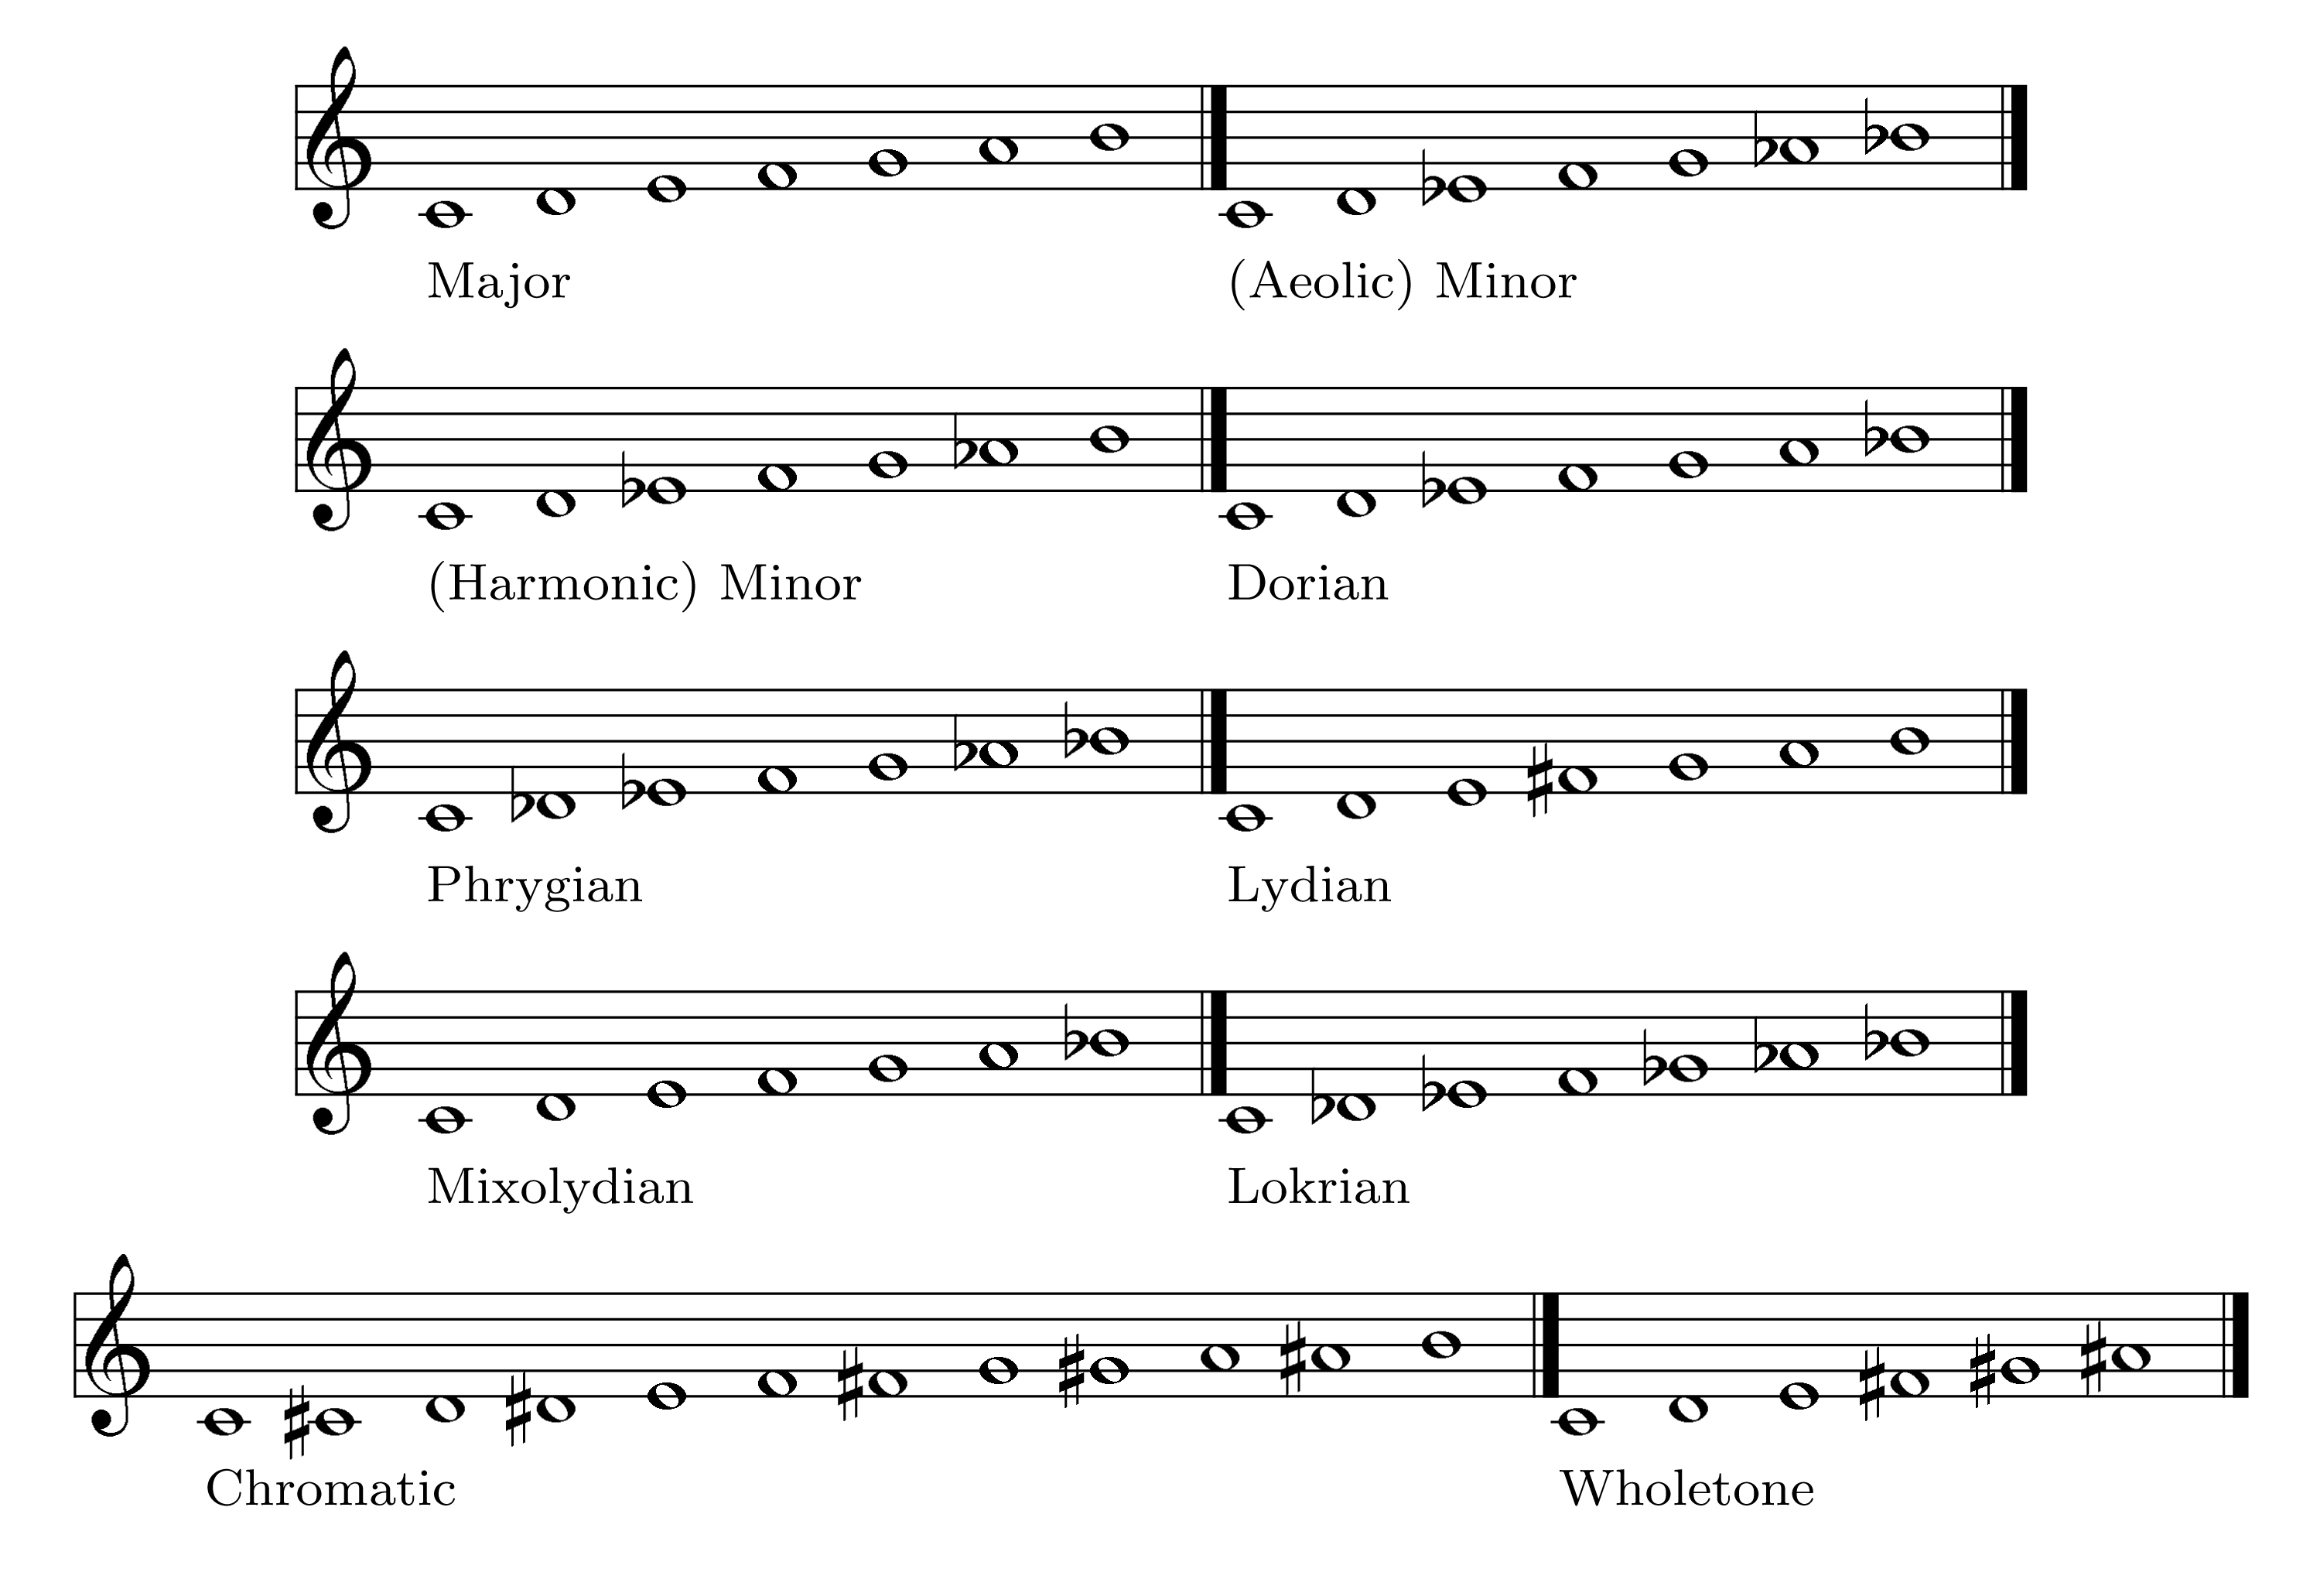
\includegraphics[scale=.65]{graph/pitch_modes}
                \end{figure}
            \end{columns}

        \end{frame}
        
        \begin{frame}{key}{key \& key signature 1/2}
            \begin{itemize}
                \item	\textbf{key}:\\ defined by \textit{tonic} (root note) and \textit{mode}
                        
                        \begin{itemize}
                            \item<1->	defines a set of pitch classes constructing both  pitch and harmonic content
                            
                        \end{itemize}
                \bigskip        
                \item<2->	\textbf{modulation} (local key changes):\\ common in various styles, uncommon in others
                \bigskip        
                \item<3->	\textbf{key signature}:\\ indicates current key with accidentals (score notation)
            \end{itemize}
        \end{frame}
        
        \begin{frame}{key}{key \& key signature 2/2}
            \vspace{-3mm}
                \begin{figure}[t]
                    \centering
                    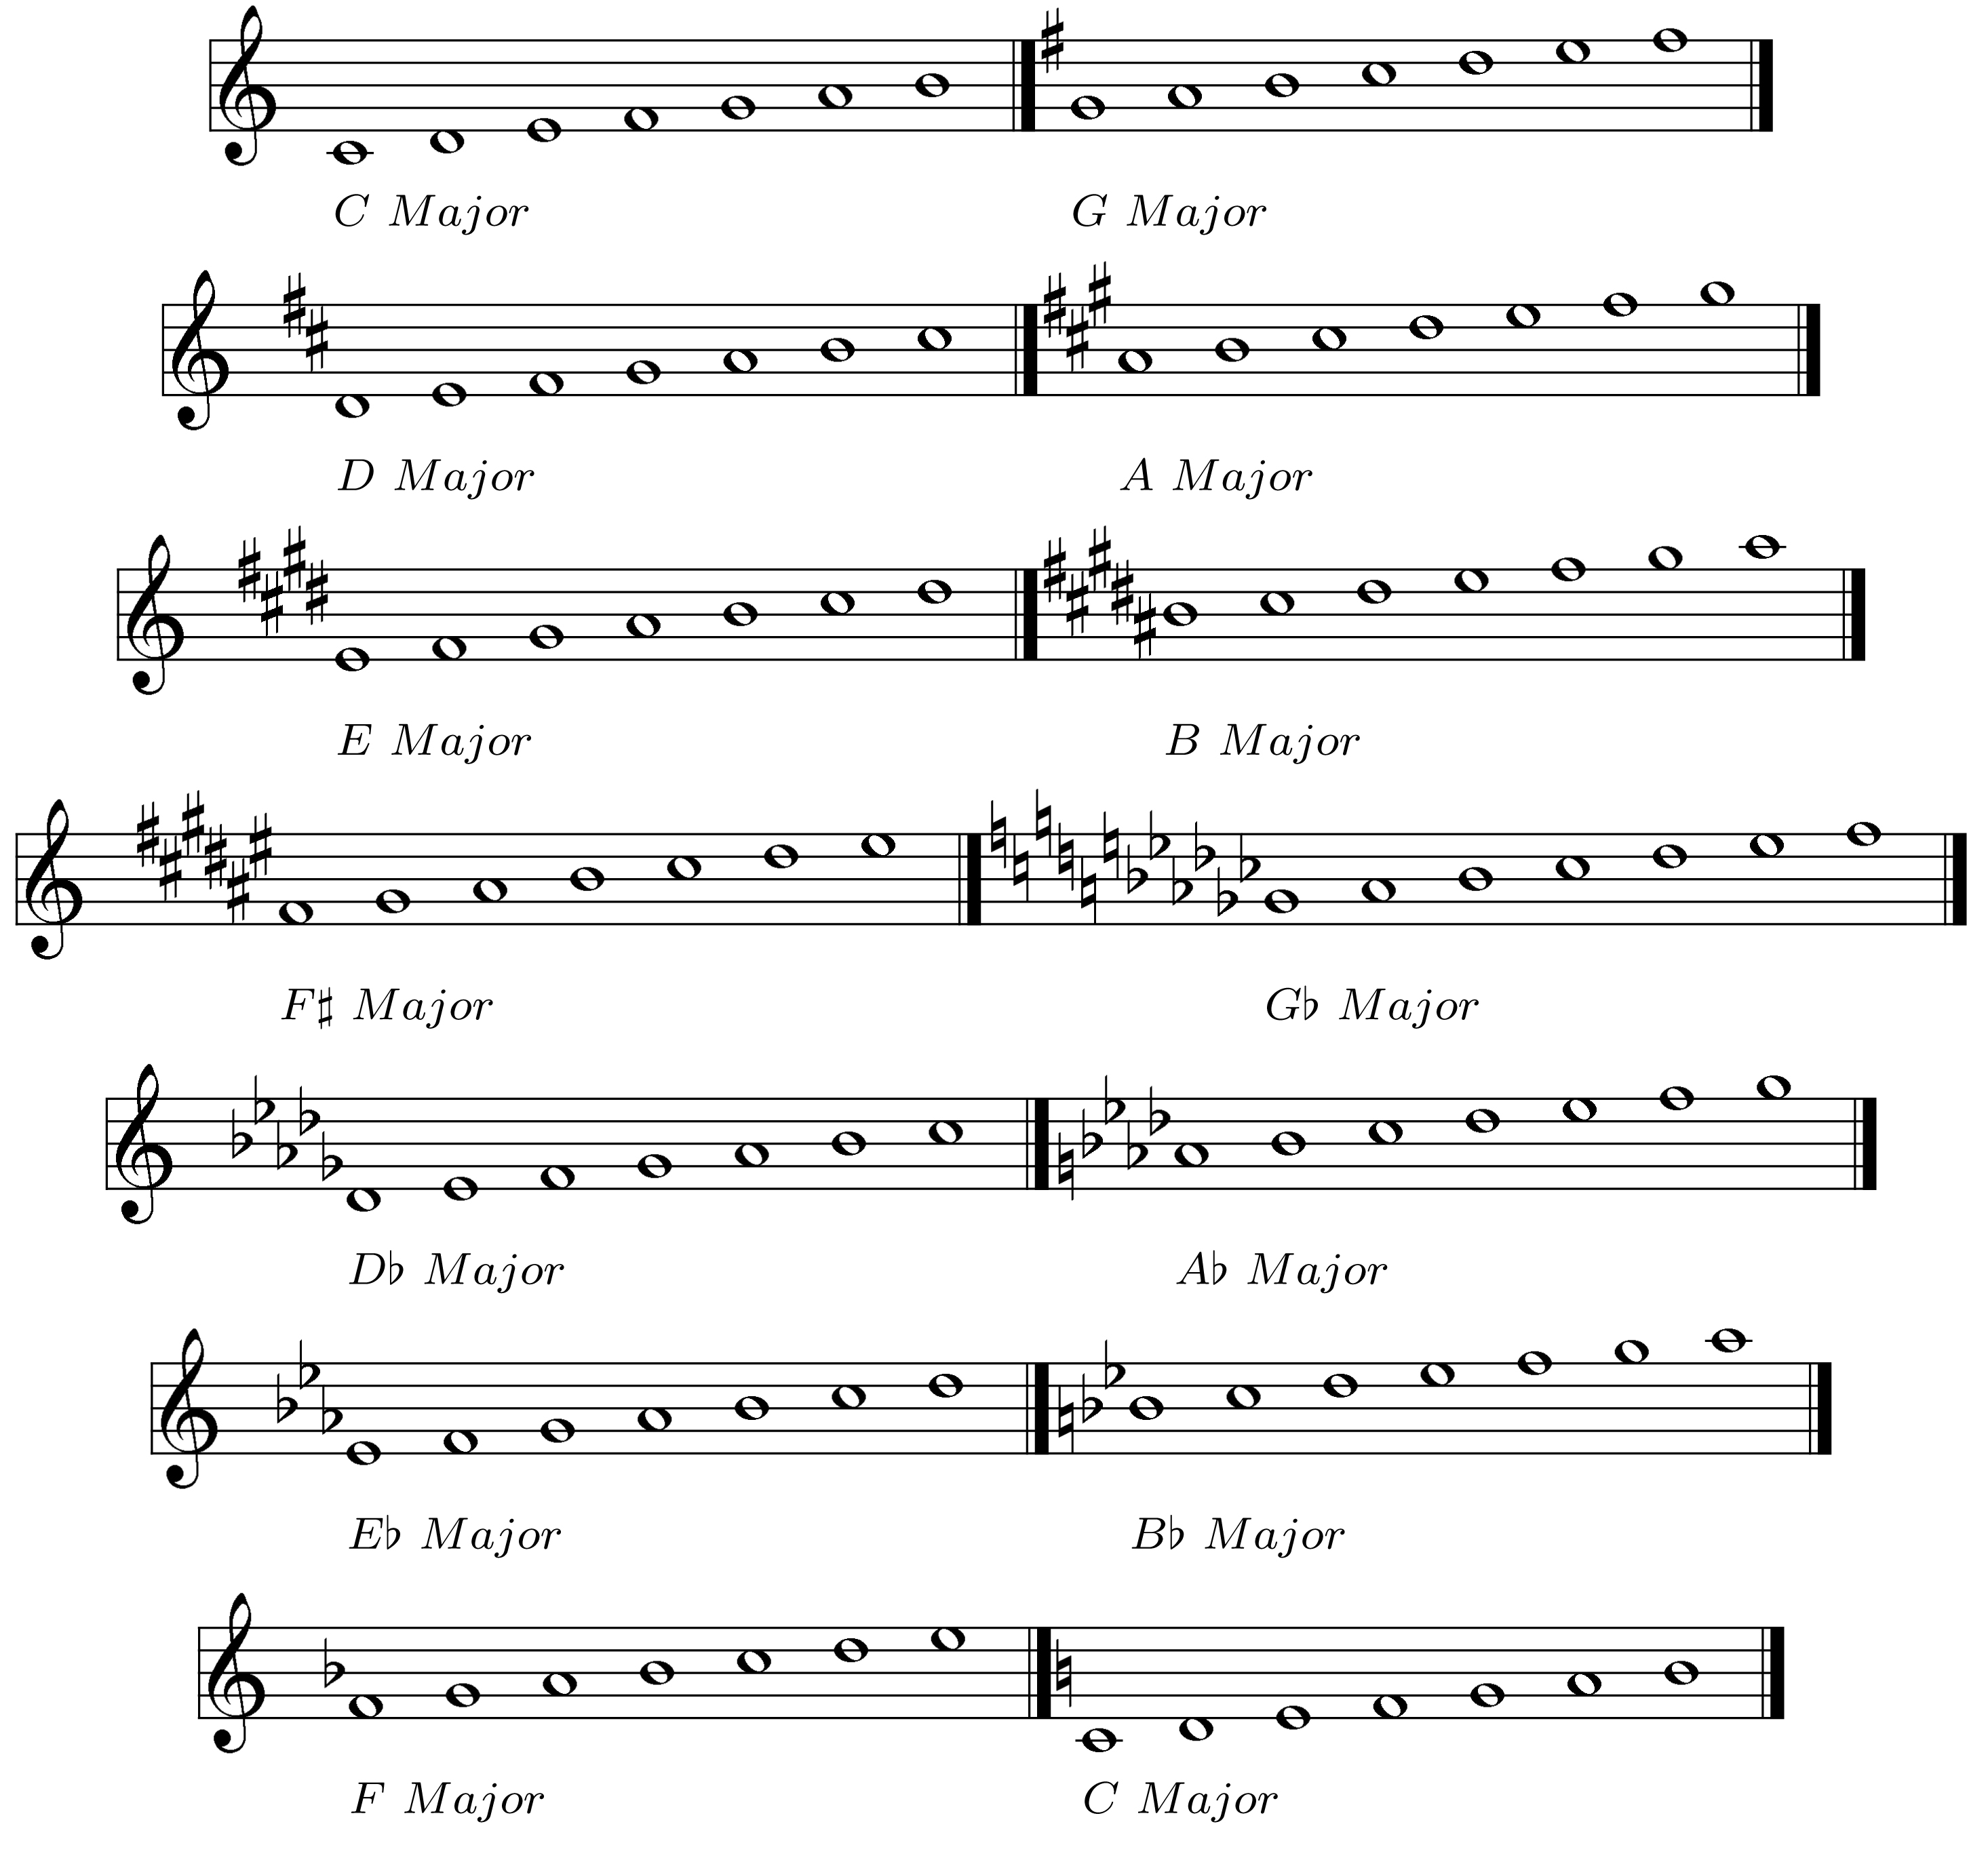
\includegraphics[scale=.6]{graph/pitch_keys}
                \end{figure}
        \end{frame}
        
        \begin{frame}{musical pitch}{key: circle of fifths}
            \vspace{-9mm}
            \begin{figure}
            \scalebox{.9}
            {
                    \centering
                    
\begin{footnotesize}
\begin{picture}(80,85)
	\setcounter{iXOffset}{40} %radius
	\setcounter{iXBlockSize}{80}

	% circles
	\put(\value{iXOffset},\value{iXOffset}){\color[rgb]{0.8,0.8,0.8}\circle*{\value{iXBlockSize}}}
	\put(\value{iXOffset},\value{iXOffset}){\color[rgb]{0.5,0.5,0.5}\circle*{58}}
	\put(\value{iXOffset},\value{iXOffset}){\color[rgb]{0.8,0.8,0.8}\circle*{36}}
	
	\put(\value{iXOffset},\value{iXOffset}){\circle{\value{iXBlockSize}}}
	\put(\value{iXOffset},\value{iXOffset}){\circle{58}}
	\put(\value{iXOffset},\value{iXOffset}){\circle{36}}

	% radial lines	
	\put( 1.363, 29.6472){\line(0.9659, 0.2588){77.3}}
	\put( 1.363, 50.3528){\line(0.9659,-0.2588){77.3}}
	
	\put( 11.7157, 11.7157){\line(0.7071, 0.7071){56.5}}
	\put( 11.7157, 68.2843){\line(0.7071,-0.7071){56.5}}
	
	\put( 29.6472, 1.3630){\line(0.2588, 0.9659){20.7}}
	\put( 29.6472, 78.6370){\line(0.2588,-0.9659){20.7}}

	% major
	\put(37.5, 78){\text{\tiny{Major}}}
	
	\put(39, 73){\text{$C$}}

	\put(56, 68){\text{$G$}}
	\put(20, 68){\text{$F$}}

	\put(68, 55){\text{$D$}}
	\put(9, 55){\text{$B\flat$}}

	\put(73, 39){\text{$A$}}
	\put(4, 39){\text{$E\flat$}}

	\put(68, 23){\text{$E$}}
	\put(9, 22){\text{$A\flat$}}

	\put(56, 10){\text{$B$}}
	\put(20, 10){\text{$D\flat$}}

	\put(36, 5){\text{$G\flat\ / F\sharp$}}


	% minor
	\put(37.5, 67){\text{\tiny{minor}}}
	
	\put(39, 63){\text{$a$}}

	\put(51, 60){\text{$e$}}
	\put(28, 60){\text{$d$}}

	\put(60, 51){\text{$b$}}
	\put(19, 51){\text{$g$}}

	\put(62, 39){\text{$f\sharp$}}
	\put(16, 39){\text{$c$}}

	\put(60, 27.5){\text{$c\sharp$}}
	\put(19, 27){\text{$f$}}

	\put(51, 19){\text{$g\sharp$}}
	\put(27, 18){\text{$b\flat$}}

	\put(37, 15){\text{$e\flat\ / d\sharp$}}

	% accidentals

	\put(38.5, 56){\text{\tiny{accs.}}}

	\put(39, 51){\text{$0$}}

	\put(45, 50){\text{$1\sharp$}}
	\put(32.5, 49.5){\text{$1\flat$}}

	\put(50, 45){\text{$2\sharp$}}
	\put(28, 45){\text{$2\flat$}}

	\put(51, 39){\text{$3\sharp$}}
	\put(27, 39){\text{$3\flat$}}

	\put(49, 33){\text{$4\sharp$}}
	\put(28, 33){\text{$4\flat$}}

	\put(45, 29){\text{$5\sharp$}}
	\put(32.5, 29){\text{$5\flat$}}

	\put(39, 28){\text{$6\flat$}}
	\put(39, 25){\text{$6\sharp$}}
	
\end{picture}
\end{footnotesize}

                
            }	
            \end{figure}
        \end{frame}
        
    \section[pitch chroma]{pitch chroma}
        \begin{frame}{pitch chroma}{introduction}
            \begin{columns}
            \column{.4\linewidth}
                \begin{itemize}
                    \item	pitch class distribution 
                    \item	12-dimensional vector
                \end{itemize}
                \begin{itemize}
                    \item	\textbf{no} octave information
                        \begin{itemize}
                            \item	robust representation
                            \item	no differentiation between unison and octave
                        \end{itemize}
                \end{itemize}
                \includeaudio{sax_example}
            \column{.6\linewidth}
                \figwithmatlab{PitchChroma}
                
            \end{columns}
        \end{frame}
        \begin{frame}{pitch chroma}{computation 1/2}
            \begin{enumerate}
                \item	divide spectral representation into \textbf{semi-tone bands}
                \item<2->	compute \textbf{mean per band}
                    \begin{footnotesize}
                        \begin{equation*}
                            \mu(j,n)		= \frac{1}{k_{\mathrm{u}}(j)-k_{\mathrm{l}}(j)+1}\sum\limits_{k=k_{\mathrm{l}}(j)}^{k_{\mathrm{u}}(j)}{|X(k,n)|^2}
                        \end{equation*}
                    \end{footnotesize}
                \item<3->	sum/mean every 12th band
                    \begin{footnotesize}
                        \begin{eqnarray*}
                            \nu(j\% 12 ,n)		&=& \sum\limits_{o=o_l}^{o_u}{\mu(j,n)}\label{eq:pc}, \\
                            \vec{\nu}(n) 	&=& \left[\nu(0,n),\, \nu(1,n),\, \nu(2,n),\, \ldots,\, \nu(10,n),\, \nu(11,n)\right]^\mathrm{T} \nonumber
                        \end{eqnarray*}
                    \end{footnotesize}
            \end{enumerate}
        \end{frame}
        \begin{frame}{pitch chroma}{computation 2/2}
            \figwithmatlab{PitchChromaGrouping}
        \end{frame}
        \begin{frame}{pitch chroma}{computation: simple variants}
            \begin{columns}
            \column{.4\linewidth}
            \begin{itemize}
                \item	\textbf{STFT}: 
                    \begin{itemize}
                        \item   \textit{weighted} mean of bins (window function)
                        \item	\textit{tonalness preprocessing} (local maxima etc)
                    \end{itemize}
                    
                \item<2->	sum of \textbf{filterbank} output energies
                   
                \item<3->	\textbf{CQT}: 
                    \begin{itemize}
                        \item sum of bins/peaks
                    \end{itemize}
                \item<4->   beat-synchronous chroma
            \end{itemize}
            
            \column{.6\linewidth}
                \only<1>{
                    \figwithmatlab{PitchChromaGrouping}
                }
                \only<2>{
                    \figwithmatlab{ResonanceFilterBank}
                }
            \end{columns}
        \end{frame}
        \begin{frame}{pitch chroma}{normalization}
            \begin{columns}[T]
                \column{.6\textwidth}
                    \begin{itemize}
                        \item   pitch chroma as \textit{distribution}:
                            \begin{equation*}
                                \sum\limits_{k=0}^{11}{\nu(k,n)} = 1
                            \end{equation*}
                        \item<2->   pitch chroma as \textit{vector}:
                            \begin{equation*}
                                \sqrt{\sum\limits_{k=0}^{11}{\nu(k,n)^2}} = 1
                            \end{equation*}
                        \item<3-> other options:
                            \begin{itemize}
                                \item   e.g., short-term energy normalization (CENS)
                            \end{itemize}
                    \end{itemize}
                \column{.4\textwidth}
                    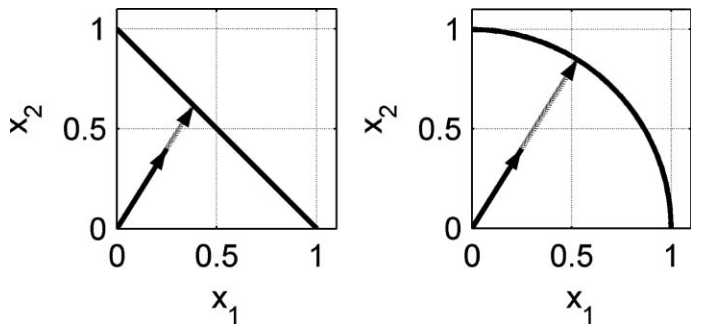
\includegraphics[scale=.2]{graph/pc-norm}
            \end{columns}
            
        \end{frame}
        
        \begin{frame}{pitch chroma}{problem 1: amplitude distortion}
            \vspace{-3mm}
            \figwithmatlab{PitchChromaLeakage}
            \begin{itemize}
                \item	every pitch contains not only fundamental but higher harmonics
                    \begin{itemize}
                        \item<2->	[$\Rightarrow$]	de-emphasize higher frequencies
                        \item<2->	[$\Rightarrow$]	build amplitude model
                        \item<2->	[$\Rightarrow$]	use multi-pitch detection system
                    \end{itemize}
            \end{itemize}
        \end{frame}
        \begin{frame}{pitch chroma}{problem 2: frequency distortion}
            \begin{itemize}
                \item	higher harmonics are not ``in-tune''
                \begin{table}
                    \centering
                    \begin{tabular}{cccccccccccc} %{\textwidth}{@{\extracolsep{\fill}}ccccccccccccc}
                        \\ \hline
                        \bf{\emph{Harmonic}}	 & \bf{\emph{$|\Delta C(f,f_T)|$}}\\ 
                         \hline
                        \bf{$f = f_0$}	 & 0\\
                        \bf{$f = 2\cdot f_0$}	 & 0\\
                        \bf{$f = 3\cdot f_0$}	 & 1.955\\
                        \bf{$f = 4\cdot f_0$}	 & 0\\
                        \bf{$f = 5\cdot f_0$}	 & 13.6863\\
                        \bf{$f = 6\cdot f_0$}	 & 1.955\\
                        \bf{$f = 7\cdot f_0$}	 & 31.1741\\
                        \hline
                        \bf{$\mu_{|\Delta C|}$}	 & 6.9672\\
                    \end{tabular}
                \end{table}
            \end{itemize}
        \end{frame}

    \section{key detection}
        \begin{frame}{key detection}{introduction}
            assumption: 
            \begin{itemize}
                \item \textit{pitch class distribution} is prototypical for key
                    \begin{itemize}
                        \item	tonic/root note is tonal center
                        \item	tonal and harmonic relations define importance and occurrence of individual pitch classes
                        \item   different root notes result in simple shift of distribution
                    \end{itemize}
            \end{itemize}
        \end{frame}
        \begin{frame}{key detection}{processing steps of simple key detection}
            \begin{columns}
                \column{.4\linewidth}
                    \begin{enumerate}
                        \item<1->	define reference distribution for specific keys
                        \item<2->	extract average pitch chroma from audio
                        \item<3->	compute distance between template and extracted chroma
                    \end{enumerate}
                \column{.6\linewidth}
                    \only<1-2>{\figwithmatlab{KeyProfileKrumhansl}}
                    \only<3>{            
                    \begin{figure}
                        \begin{center}
                        \begin{picture}(60,25)
                
                            %boxes
                            \put(0,10){\ovalbox{\footnotesize{\parbox{20mm}{\centering{extracted\\ pitch chroma}}}}}
                            \put(0,20){\ovalbox{\footnotesize{\parbox{20mm}{\centering{template\\ pitch chroma}}}}}
                            \put(27,15){\ovalbox{\footnotesize{\parbox{20mm}{\centering{distance measure}}}}}
                
                        
                            %diagonal
                            \put(22.5,11){\vector(1,1){4.5}}
                            \put(22.5,21){\vector(1,-1){4.5}}
                            
                            % horizontal
                            \put(49,15.5){\vector(1,0){10}}
                
                            %text
                            \put(54,16){\footnotesize{\shortstack[c]{key}}}
                
                        \end{picture}
                        \end{center}
                    \end{figure}
                    }
            \end{columns}
        \end{frame}
        \begin{frame}{key detection}{key template distance animation}
            \includeanimation{KeyDetection}{01}{12}{1}
        \end{frame}
        
        \begin{frame}{key detection}{key templates}
            \vspace{-5mm}
            \begin{columns}
            \column{.4\linewidth}
                    \begin{itemize}
                        \item	\emph{Orthogonal} $\vec{\nu}_\mathrm{o}$: root note is most salient component, other components negligible
                                \pause
                                \begin{itemize}
                                    \item	same distance to all keys
                                    \item	no major/minor distinction 
                                \end{itemize}
                        %\item<2->	\emph{Smoothed Orthogonal} $\vec{\nu}_\mathrm{s}$:  root note most salient, neighboring components less important
                                %\pause
                                %\begin{itemize}
                                    %\item	increasing key distance to tritone
                                    %\item	no real distinction between major and minor
                                %\end{itemize}
                        \item<3->	\emph{Diatonic} $\vec{\nu}_\mathrm{d}$: all key-inherent pitches weighted equally
                                \pause
                                \begin{itemize}
                                    \item	linear increasing key dist
                                \end{itemize}
                        \item<4->	\emph{Probe tone Ratings}  $\vec{\nu}_\mathrm{p}$: derived from perceptual tonal similarity
                        \item<5->	\emph{Extracted Key Profiles} $\vec{\nu}_\mathrm{t}$: derived from real-world data
                    \end{itemize}
            \column{.6\linewidth}
                \vspace{-5mm}
                \figwithmatlab{KeyProfiles}
                \vspace{20mm}
            \end{columns}
        \end{frame}
        %\begin{frame}{key detection}{key templates 2/2}
            %\figwithmatlab{KeyProfiles}
        %\end{frame}
        %\begin{frame}{key detection}{distance measures: (vector) distance}
            %\begin{footnotesize}
                    %\begin{itemize}
                        %\item	\emph{{Euclidean distance}}:
                                %$d_\mathrm{E}(s) = \sqrt{\sum\limits_{j = 0}^{11}{\big(\nu_\mathrm{e}(j)-\nu_\mathrm{t,s}(j)\big)^2}} $
                        %\item<2->	\emph{{Manhattan distance}}:
                                %$d_\mathrm{M}(s) = \sum\limits_{j = 0}^{11}{\big|\nu_\mathrm{e}(j)-\nu_\mathrm{t,s}(j)\big|} $
                        %\item<3->	\emph{{Cosine distance}}:
                                %$d_\mathrm{C}(s) = 1-\left( \frac{\sum\limits_{j = 0}^{11}{\nu_\mathrm{e}(j)\cdot\nu_\mathrm{t,s}(j)}}{\sqrt{\sum\limits_{j = 0}^{11}{\nu_\mathrm{e}(j)^2}}\sqrt{\cdot \sum\limits_{j = 0}^{11}{\nu_\mathrm{t,s}(j)^2}}}\right) $
                        %\item<4->	\emph{{Kullback-Leibler divergence}}:
                                %$d_\mathrm{KL}(s) = \sum\limits_{j = 0}^{11}{\nu_\mathrm{e}(j)\cdot\log\left(\frac{\nu_\mathrm{e}(j)}{\nu_\mathrm{t,s}(j)}\right)}$
                        %\item<5->   \textit{nearest neighbor classification}
                    %\end{itemize}
            %\end{footnotesize}
        %\end{frame}
        %%\begin{frame}{key detection}{distance measures: k-Nearest Neighbor}
            %%\begin{itemize}
                %%\item	\textbf{training}: extract reference vectors from training set (keep class labels)
                %%\pause
                %%\item	\textbf{classification}: extract test vector and set class to majority of $k$ nearest reference vectors
            %%\end{itemize}
                %%\begin{figure}[t]
                    %%\centering
                        %%\includegraphics[scale=.7]{graph/KnnClassification}
                %%\end{figure}
        %%\end{frame}
        \begin{frame}{key detection}{variants}
            \begin{itemize}
                \item	\textbf{tonalness weight}:\\ estimate the tonality/noisiness and weight instantaneous pitch chroma
                \item<2->	\textbf{multiple estimations}:\\ split piece into regions and estimate key through majority
                \item<3->	\textbf{real-time key detection}:\\ estimate in sliding window
            \end{itemize}
        \end{frame}
        \begin{frame}{key detection}{results \& typical errors}
            \begin{columns}[T]
            \column{.6\textwidth}
                \begin{itemize}
                    \item	typical errors: related keys
                        \begin{itemize}
                            \item	Dominant
                            \item	Subdominant
                            \item	Relative
                            \item	Major/Minor
                        \end{itemize}
                \end{itemize}
            \column{.4\textwidth}
                \begin{figure}
                    \centering
                        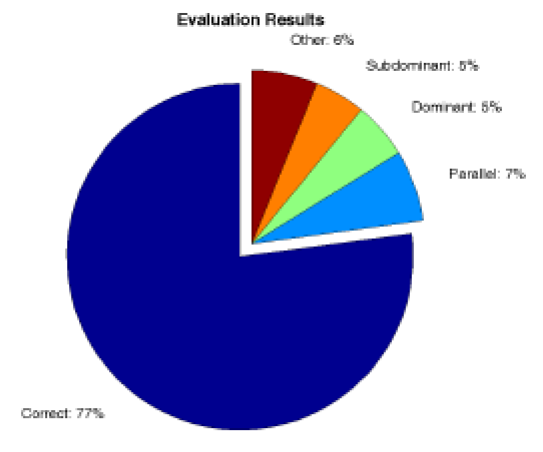
\includegraphics[scale=.35]{graph/resultskeydetection}
                \end{figure}
            \end{columns}
            \begin{flushright}
                graph from \footfullcite{lerch_ansatz_2004}
            \end{flushright}
        \end{frame}
                
    \section{summary}
        \begin{frame}{summary}{lecture content}
            \begin{itemize}
                \item   \textbf{musical key}
                    \begin{itemize}
                        \item   set of pitch classes constructing pitched content
                        \item   defined by \textit{tonic} (important center) and \textit{mode} (scale)
                    \end{itemize}
                \bigskip
                \item   \textbf{pitch chroma}
                    \begin{itemize}
                        \item   reduced 12-dimensional octave-independent pitch representation
                        \item   relatively robust against timbre variation
                    \end{itemize}
                \bigskip
                \item   \textbf{automatic key recognition}
                    \begin{itemize}
                        \item   standard approach is template-based
                        \item   extracted average pitch chroma is compared with predefined template
                        \item   inverse distance measure indicates key likelihoods
                    \end{itemize}
            \end{itemize}
            \inserticon{summary}
        \end{frame}
\end{document}
